 \documentclass[onecolumn,11pt]{article}
%*********
%Paquetes
%*********
\usepackage[spanish]{babel}
\usepackage[utf8]{inputenc}
\usepackage[a4paper, total={7in, 9in}]{geometry}
\usepackage{amsfonts}
\usepackage{dsfont}
\usepackage{physics}
\usepackage{xcolor}
\usepackage{tikz-cd} %para diagrama conmutatitvo
\usepackage{multicol} %para la lista de operadores
\usepackage{hyperref}
\usepackage{caption}
\usepackage{subcaption} %para las subfiguras
\title{Evolución del SWAP y estado de máxima entropía}
%*********
%Comandos
%*********
\newcommand{\mcU}{\mathcal{U}}
\newcommand{\mcO}{\mathcal{O}}
\newcommand{\mcI}{\mathcal{I}}
\newcommand{\mcL}{\mathcal{L}}
\newcommand{\mcS}{\mathcal{S}}
\newcommand{\hilbert}{{\sf H}}
\newcommand{\mcB}{\mathcal{B}}
\newcommand{\mcH}{\mathcal{H}}
\newcommand{\mcF}{\mathcal{F}}
\newcommand{\mcC}{\mathcal{C}}
\newcommand{\mcT}{\mathcal{T}}
\newcommand{\mcE}{\ensuremath{\mathcal{E}} }
\newcommand{\mcG}{\ensuremath{\mathcal{G}} }
\newcommand{\mcM}{\mathcal{M}}
\newcommand{\mcN}{\mathcal{N}}
\newcommand{\nnn}{\mathcal{N}}
\newcommand{\choi}{\ensuremath{\mcD} }
\newcommand{\mmm}{\mathcal{M}}
\newcommand{\sss}{\mathcal{S}}
\newcommand{\mcD}{\mathcal{D}}
\newcommand{\mcA}{\mathcal{A}}
\newcommand{\mcP}{\mathcal{P}}
\newcommand{\Complex}{\mathbb{C}} %Para escribir al espacio de hilbert complejo
\newcommand{\Id}{\mathds{1}}% Para escribir el op. indentidad con notación chida
\newcommand{\CG}[1]{\mcC\left[#1\right]}
\newcommand{\Fuzzy}[1]{\mcF\left[#1\right]}
\newcommand{\nota}[1]{{\color{red} [#1]}}
\newcommand{\notaAd}[1]{{\color{blue} [#1]}} %Notas pero mías
\graphicspath{ {../figures/} }
\begin{document}
\maketitle
\thispagestyle{empty}
\section{Parte analítica}
\subsection{Una unitaria para gobernarlos a todos}

Un operador unitario se traduce como una rotación en la esfera de Bloch. Entonces dos operadores están relacionados por una unitaria si sus vectores de Bloch tienen la misma norma (esto es, los operadores tienen la misma norma de Frobenius).

Si consideramos un estado sobre el eje z,

\begin{equation}
\rho_{z}=\frac{1}{2}\qty(\Id+z\sigma_{z})
\end{equation}

entonces este está relacionado mediante una unitaria a cualquier estado $\rho$ con vector de Bloch $\vec{r}$ tal que $\abs{\vec{r}}=z$.

\subsection{El grueso rotado es igual al grueso del rotado}
Sea $\rho_{z}$ un estado grueso sobre z definido como antes, y sea $\{\psi_{i}\}_{i=1}^{N}$ el conjunto de estados con los que se obtiene su estado fino asignado. Además, sea $\rho$ un estado grueso tal que $\abs{\vec{r}}=z$.

\begin{equation}
\Rightarrow \exists U \text{ tal que } U\rho_{z}U^{\dag}=\rho
\end{equation}

Sea $\mcU=U\otimes U$, $\sigma_{i}'=U\sigma_{i}U^{\dag}$. En las siguientes líneas se muestra que si se rota a todo el conjunto $\{\psi_{i}\}$ usando $\mcU$, lo que se halla es el conjunto fino para el mapeo de asignación de $\rho$. Nótese que la rotación no modifica la distribución de los estados siempre que estos satisfagan la medida de Haar.

\begin{align*}
\CG{\mcU \psi_{i} \mcU^{\dag}}=&\Tr_{2}\qty[p\mcU\psi_{i}\mcU^{\dag}+(1-p)S\mcU \psi_{i} \mcU^{\dag}S^{\dag}]\\
=&\Tr_{2}\qty[p\mcU\qty(\frac{1}{4}\sum_{i,j}\gamma_{ij} \sigma_i\otimes\sigma_j)\mcU^{\dag}+(1-p) S\mcU \qty(\frac{1}{4}\sum_{i,j}\gamma_{ij} \sigma_i\otimes\sigma_j) \mcU^{\dag} S^{\dag}]\\
=&\Tr_{2}\qty[p\qty(\frac{1}{4}\sum_{i,j}\gamma_{ij} \sigma_{i}'\otimes\sigma_{j}')+(1-p)S \qty(\frac{1}{4}\sum_{i,j}\gamma_{ij} \sigma_{i}'\otimes\sigma_{j}')S^{\dag}]\\
=&\Tr_{2}\qty[p\qty(\frac{1}{4}\sum_{i,j}\gamma_{ij} \sigma_{i}'\otimes\sigma_{j}')+(1-p)\qty(\frac{1}{4}\sum_{i,j}\gamma_{ij} \sigma_{j}'\otimes\sigma_{i}')]\\
\end{align*}
\begin{align*}
\Rightarrow\CG{\mcU \psi_{i} \mcU^{\dag}}=&\frac{1}{2}\qty[\Id +p\sum_{i=1}\gamma_{i,0}\sigma_{i}'+(1-p)\sum_{j=1}\gamma_{0,j}\sigma_{j}']\\
=&\frac{1}{2}\qty[\Id + \sum_{i=1}^3[p\gamma_{i,0}+(1-p)\gamma_{0,i}]U\sigma_{i}U^{\dag}]\\
=&U\frac{1}{2}\qty[\Id + \sum_{i=1}^3[p\gamma_{i,0}+(1-p)\gamma_{0,i}]\sigma_{i}]U^{\dag}\\
=&U\CG{\psi_{i}}U^{\dag}\\
=&U\rho_{z}U^{\dag}\\
\end{align*}
Como esto es para todo $i$, si se rota cada $\psi_{i}$, lo que obtenemos es un conjunto que podemos promediar para hallar el estado fino asignado a $\rho$. Aún mejor, como el promedio es lineal:
\begin{align}
\mcA[\rho]=&\frac{1}{N}\sum_{i}U\psi_{i}U^{\dag}\\
=&U\qty(\frac{1}{N}\sum_{i}\psi_{i})U^{\dag}\\
=&U\mcA[\rho_{z}]U^{\dag}
\end{align}
Esto significa que podemos hallar el mapeo de asignamiento de un estado $\rho$ a través del mapeo de asignamiento de otro estado $\rho_{z}$, siempre y cuando exista una unitaria entre estos.
\subsection{Para el MaxEnt es lo mismo pero no es igual}
Considérese un estado grueso $\rho_{c}\in \mcL(\mcH_{2})$, y sea $\psi\in\mcL(\mcH_{4})$ su estado subyacente $\CG{\psi}=\rho_{c}$. Si el observador puede realizar mediciones de $\sigma_{i}$ en el estado grueso, entonces es posible reconstruir un estado de máxima entropía $\psi_{max}$ según
\begin{equation}\label{eq:MaxEnt}
\psi_{max}=\frac{1}{\Tr(e^{\sum_{i}\lambda_{i}\hat{G}_{i}})}e^{\sum_{i}\lambda_{i}\hat{G}_{i}}
\end{equation}
donde $\lambda_{i}$ son los multiplicadores de Lagrange y $\hat{G}_{i}$ son operadores no tomográficamente completos \cite{MaxEnt}. Se puede demostrar que los operadores $\hat{G}_{i}$ son
\begin{equation}\label{eq:Gop}
\hat{G}_{i}=p\sigma_{i}\otimes\Id+(1-p)\Id\otimes\sigma_{i}
\end{equation}

Idealmente, la ecuación (\ref{eq:MaxEnt}) está en términos de los valores de expectación $r_{i}=Tr(\sigma_{i}\rho_{c})$, y no de los multiplicadores de Lagrange. Para simplificar el problema, se puede asumir que $\rho_{c}$ está alineado con el eje $z$, de tal forma que el exponente en (\ref{eq:MaxEnt}) tenga únicamente un término.

\vspace{0.2cm}

En las siguientes líneas se demuestra que para todo $\rho_{c}$ con vector de Bloch $\vec{r}$ es posible reconstruir el estado de máxima entropía a través del estado de máxima entropía asociado a un estado grueso alineado en $z$, $\rho_{z}$ y la unitaria $U$ que relaciona $\rho_{c}$ y $\rho_{z}$ (para que esta exista se debe cumplir que $\abs{\vec{r}}=z$).

\vspace{0.2cm}

Sea, pues $\rho_{c}$ tal que $\rho_{c}=U\rho_{z}U^{\dag}$, con $\psi_{max}$ el estado de máxima entropía reconstruído para  $\mcU=U\otimes U$. El valor de expectación de las $\sigma_{i}$ puede calcularse como
\begin{align*}
r_{i}&=\Tr\{\sigma_{i}U\rho_{z}U^{\dag}\}\\
&=\Tr\{\sigma_{i}U\CG{\psi_{z}}U^{\dag}\}\\
&=\Tr\{\sigma_{i}\CG{\mcU\psi_{z}\mcU^{\dag}}\}\\
&=\Tr\{\Tr_{2}[\sigma_{i}\otimes\Id(p\mcU\psi_{z}\mcU^{\dag}+(1-p)S\mcU\psi_{z}\mcU^{\dag}S)]\}\\
&=\Tr[\sigma_{i}\otimes\Id(p\mcU\psi_{z}\mcU^{\dag}+(1-p)S\mcU\psi_{z}\mcU^{\dag}S)]\\
&=\Tr[p\mcU^{\dag}(\sigma_{i}\otimes\Id)\mcU\psi_{z}+(1-p)\mcU^{\dag}S(\sigma_{i}\otimes\Id) S\mcU\psi_{z}]\\
&=\Tr[p\mcU^{\dag}(\sigma_{i}\otimes\Id)\mcU\psi_{z}+(1-p)\mcU(\Id\otimes\sigma_{i})]\\
&=\Tr[\mcU^{\dag}(p\sigma_{i}\otimes\Id+(1-p)\Id\otimes\sigma_{i})\mcU\psi_{z}]\\
&=\Tr[\mcU^{\dag}\hat{G}_{i}\mcU\psi_{z}]\\
\end{align*}
De esto, se sigue que el estado de máxima entropía se recontruye como:
\begin{align*}
\psi_{max}&=\frac{1}{\Tr(e^{\sum_{i}\lambda_{i}\mcU^{\dag}\hat{G}_{i}\mcU})}e^{\sum_{i}\lambda_{i}\mcU^{\dag}\hat{G}_{i}\mcU}\\
&=\frac{1}{\Tr(e^{\mcU^{\dag}\qty(\sum_{i}\lambda_{i}\hat{G}_{i})\mcU^{\dag}})}e^{\mcU^{\dag}\qty(\sum_{i}\lambda_{i}\hat{G}_{i})\mcU^{\dag}}\\
&=\frac{1}{\Tr(\mcU^{\dag}e^{\sum_{i}\lambda_{i}\hat{G}_{i}}\mcU)}\mcU^{\dag}\qty(e^{\sum_{i}\lambda_{i}\hat{G}_{i}})\mcU\\
&=\frac{1}{\Tr(\mcU^{\dag}\qty(e^{\sum_{i}\lambda_{i}\hat{G}_{i}})\mcU)}\mcU^{\dag}\qty(e^{\sum_{i}\lambda_{i}\hat{G}_{i}})\mcU\\
&=\frac{1}{\Tr(e^{\sum_{i}\lambda_{i}\hat{G}_{i}})}\mcU^{\dag}\qty(e^{\sum_{i}\lambda_{i}\hat{G}_{i}})\mcU\\
&=\mcU^{\dag}\psi_{max}\mcU
\end{align*}
\subsection{El estado de máxima entropía en términos de $r_{z}$}
Si se asume que $\rho_{z}$ es un estado grueso alineado sobre el eje z, por (\ref{eq:MaxEnt}) el estado de máxima entropía es:
\begin{equation}\label{eq:MaxEntZ}
\psi_{max}=\frac{\text{exp}(\lambda_{3}\hat{G}_{3})}{\Tr[\text{exp}(\lambda_{3}\hat{G}_{3})]}
\end{equation}
donde $\hat{G}_{3}$ se define según (\ref{eq:Gop}). La forma matricial de este estado es:
\begin{equation*}
\left(
\begin{array}{cccc}
 \frac{1}{4} e^{-\lambda_{3}} \text{sech}(\lambda_{3} p)
   \text{sech}(\lambda_{3}-\lambda_{3} p) & 0 & 0 & 0 \\
 0 & \frac{e^{2 \lambda_{3}}}{\left(e^{2 \lambda_{3}
   p}+1\right) \left(e^{2 \lambda_{3}}+e^{2 \lambda_{3}
   p}\right)} & 0 & 0 \\
 0 & 0 & \frac{1}{\left(e^{2 \lambda_{3}}+1\right) e^{-2
   \lambda_{3} p}+e^{2 \lambda_{3}-4 \lambda_{3}
   p}+1} & 0 \\
 0 & 0 & 0 & \frac{1}{4} e^{\lambda_{3}}
   \text{sech}(\lambda_{3} p) \text{sech}(\lambda_{3}-\lambda_{3} p) \\
\end{array}
\right)
\end{equation*}
Hallar el valor de $\lambda_{
3}$ en términos del valor $r_{z}$ implica resolver la ecuación:
\begin{equation}\label{eq:RZ}
rz=-\frac{1}{2}\sech{p\lambda_{3}}\sech{(1-p)\lambda_{3}}(\sinh{\lambda_{3}}+(1-p)\sinh{\lambda_{3}(1-2p)})
\end{equation}
No se ve ninguna forma sencilla de despejar al multiplicador de Lagrange. En realidad, esto solo se puede si la función $r_{z}(\lambda_{3})$ tiene inversa, y esto puede depender del parámetro $p$. Graficar la superficie puede dar algunas ideas del problema. La superficie es observable en la figura \ref{fig:rzsurf}.

Después de una breve inspección se concluyen las siguientes cosas:
\begin{itemize}
\item la superficie es simétrica respecto al plano $p=0.5$
\item la superficie es antisimétrica respecto al plano $\lambda_{3}=0$
\item $\text{sgn}(\lambda_{3})=-\text{sgn}(r_{z})$
\end{itemize}
¿Pero es posible, fijada p, hallar a $\lambda_{3}$ en función de $r_{z}$? La figura \ref{fig:rzinv} parece sugerir que claro que sí. Aún más, parece que la relación es del tipo $\lambda_{3}=\text{arctanh}(r_{z})$. Así que bueno, aunque aún no he hallado la expresión, creo que debe existir.

\begin{figure}[h!]
\centering
\begin{subfigure}{0.475\textwidth}
  \centering
  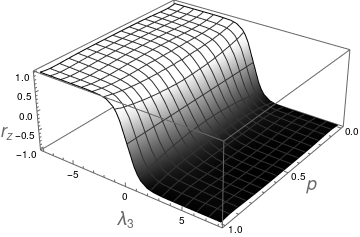
\includegraphics[width=0.6\linewidth]{LagrangeMult_lambda-8to8.png}
  \caption{$-8<\lambda_{3}<8$}
\end{subfigure}%
\begin{subfigure}{0.475\textwidth}
  \centering
  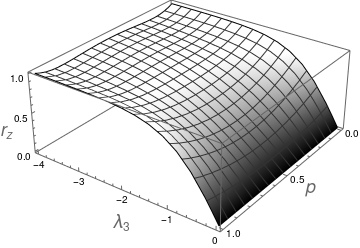
\includegraphics[width=0.6\linewidth]{LagrangeMult_lambda-4to0.png}
  \caption{$-4<\lambda_{3}<0$}
\end{subfigure}
\caption{Superficie de $r_{z}$ según (\ref{eq:RZ}) para dos intervalos de $\lambda_{3}$. A valores $\lambda_{3}<0$ corresponden valores $r_{z}>0$ y viceversa.}
\label{fig:rzsurf}
\end{figure}
\begin{figure}[h!]
\centering
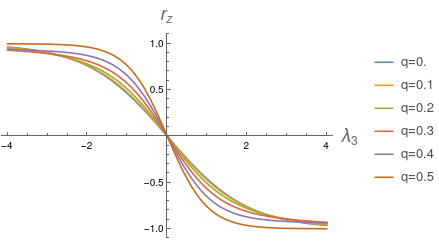
\includegraphics[width=0.6\linewidth]{rz_has_inverse_lambda-4to4.png}
\caption{$r_{z}$ como función de $\lambda_{3}$ para diferentes valores de $p$. La apariencia uno a uno sugiere la existencia de una inversa.}
\label{fig:rzinv}
\end{figure}

\section{Parte analítica}

\subsection{Numérica}
\subsubsection{Cascarón de estados mixtos}
Se generan estados puros $\begin{pmatrix}
a\\
b\\ \end{pmatrix}$ de manera uniforme. Estos son puntos en el cascarón unitario. Todos estos puntos se deplazan radialmente hacia adentro mediante un factor:
\begin{equation}
\vec{\alpha}=r\vec{\alpha_{0}}
\end{equation}
El resultado es un conjunto de estados mixtos $\{\rho_{i}\}_{i=1}^{N}$ cuyos vectores de Bloch se encuentran en el cascarón de radio $r$.

\subsubsection{Mapeo de asignación para el cascarón}


A cada $\rho_{i}$ hay que hallarle su estado fino asignado. Lo que se hace es generar un conjunto $\{\psi_{i}\}_{i=1}^{N}$ de estados finos para un estado grueso en $z$, $\rho_{z}$, tal que su coordenada en $z$ es justamente el radio del cascarón.

Como existe una unitaria $U_{i}$ entre $\rho_{z}$ y cada estado de $\{\rho_{i}\}_{i=1}^{N}$. Entonces podemos aplicar estas unitarias para hallar todos los $\mcA[\rho_{i}]$.

\subsubsection{Resultados}

Dos experimentos. En el primero se utiliza una probabilidad de swap $p=0.5$ (cascarón de radio $r=0.3$). El conjunto no cambia. En el segundo se utiliza una probabilidad de swap $p=0.3$ (cascarón de radio $r=0.8$).

Se grafican dichos cascarones en azul. Se aplica un SWAP a todos los $\mcA[\rho_{i}]$, y se saca el coarse graining. El resultado se grafica en amarillo.

\begin{figure}[h]
\centering
\begin{subfigure}{0.4\textwidth}
  \centering
  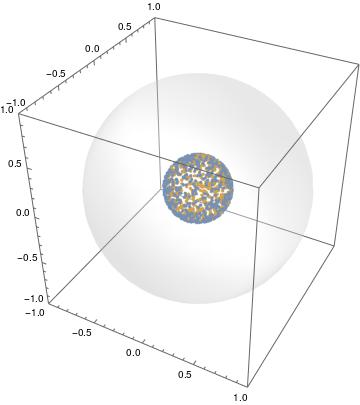
\includegraphics[width=0.8\linewidth]{figures/effectiveswap_p=0.5_z=0.3.jpeg}
  \caption{$p=0.5$, $r=0.3$, el conjunto no cambia después del swap subyacente}
  \label{fig:paralelogram}
\end{subfigure}
\begin{subfigure}{0.4\textwidth}
  \centering
  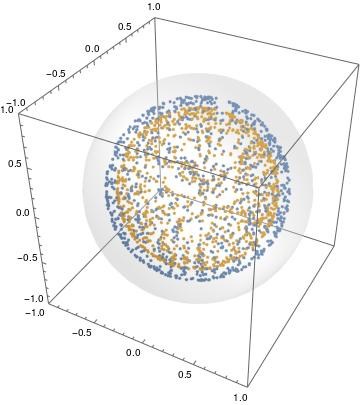
\includegraphics[width=0.8\linewidth]{figures/effectiveswap_p=0.3_z=0.8.jpeg}
  \caption{$p=0.5$, $r=0.3$, el conjunto se contrae  después del swap subyacente}
  \label{fig:paralelogram}
\end{subfigure}
\label{fig:cooldensities}
\end{figure}


\bibliographystyle{ieeetr}
\bibliography{bibliography}


\end{document}
